
\chapter{Results} \label{chapter::results}
This chapter focuses on the evaluation of the chosen empirical methods and relates back to the originally proposed research question (Section \ref{section::thesis_objective}).
Specifically, the executed performance profiling results for both apps
along the chosen metrics (see Section \ref{subsection::selected_measurement_variables}) are comparatively evaluated in order to test the validity of the performance hypothesis $H_P$ (Section \ref{section::methods}).
Furthermore, the conducted expert interviews are analysed using the process of interview coding (see Section \ref{section::interview_evaluation}) to corroborate the usability hypothesis $H_U$ (Section \ref{section::methods}).

\section{Performance Comparison} \label{section::performance_comparison}
This section presents and contextualizes the performance tracing results based on the benchmarking process for the selected metrics (detailed in Section \ref{section::performance_comparison_design}).
The section concludes with inferences of the results on the performance hypothesis $H_P$.

\subsection{General Observations}
In most cases, the iPhone 6s consumes less system resources than the iPhone 12 Pro Max (see Section \ref{section::performance_tracing_results}).
The iPhone 12 Pro Max has a considerably larger screen (6.7 inches vs. 4.7 inches) and a higher pixel density than the 6S (458 pixels/inch vs 326 pixels/inch; \cite{Apple2021d}, \cite{Apple2021c}) naturally requiring more system resources for rendering.


\subsection{CPU usage} \label{section::cpu_usage}
For both the Flutter and original iOS app, the iPhone 12 Pro Max uses more CPU power than the iPhone 6s. Furthermore, for every user action/iPhone combination, the 
CPU usage is greater than 100\%. This doesn't mean that the processing unit is overloaded as the measured CPU usage is in relation to a single core.
The iPhone 12 Pro Max has 2 high performance cores and 4 smaller battery optimized cores. Based on the task, the operating system delegates tasks to either a high performance or a 
battery optimized core.
Whereas the iPhone 6s simply has 2 equally clocked cores for typical parallel work.
In terms of CPU usage, it would be errorprone to combine values from the two different phones into a single metric. Therefore, the following metrics are calculated for the two iPhones separately.\\
Overall, the Flutter clone uses more CPU resources during every single test case when averaged over time (see Fig. \ref{fig:avg_cpu_usage_summary}) on both test hardware devices.
On average, the Flutter clone uses 43\% more CPU power when testing on the iPhone 12 Pro Max while it uses 17\% more on the iPhone 6s.\\
During the \textit{detail view transition}, the Flutter clone has the most similar CPU performance with an additional 19\% (12 Pro Max) and 14\% (6s) respectively compared to the original iOS app.

The standard deviation of the averaged CPU usage between the use cases lies between 6 and 17\% meaning that the CPU requirement for the typical use cases is similar.
Contrarily, when looking at the at each individual use case for the averaged run, the CPU usage deviation is very high in every case (app start: 48.17\%, detail transition: 53.16\%, image gallery: 51.90\%, scrolling: 52.12\%).
This should be mostly due to the fact that the CPU has different load requirements based on the current executed task which may be executed in milliseconds after which it may be idle if no other task is in the queue.

\begin{figure}[!h]
    \centering
    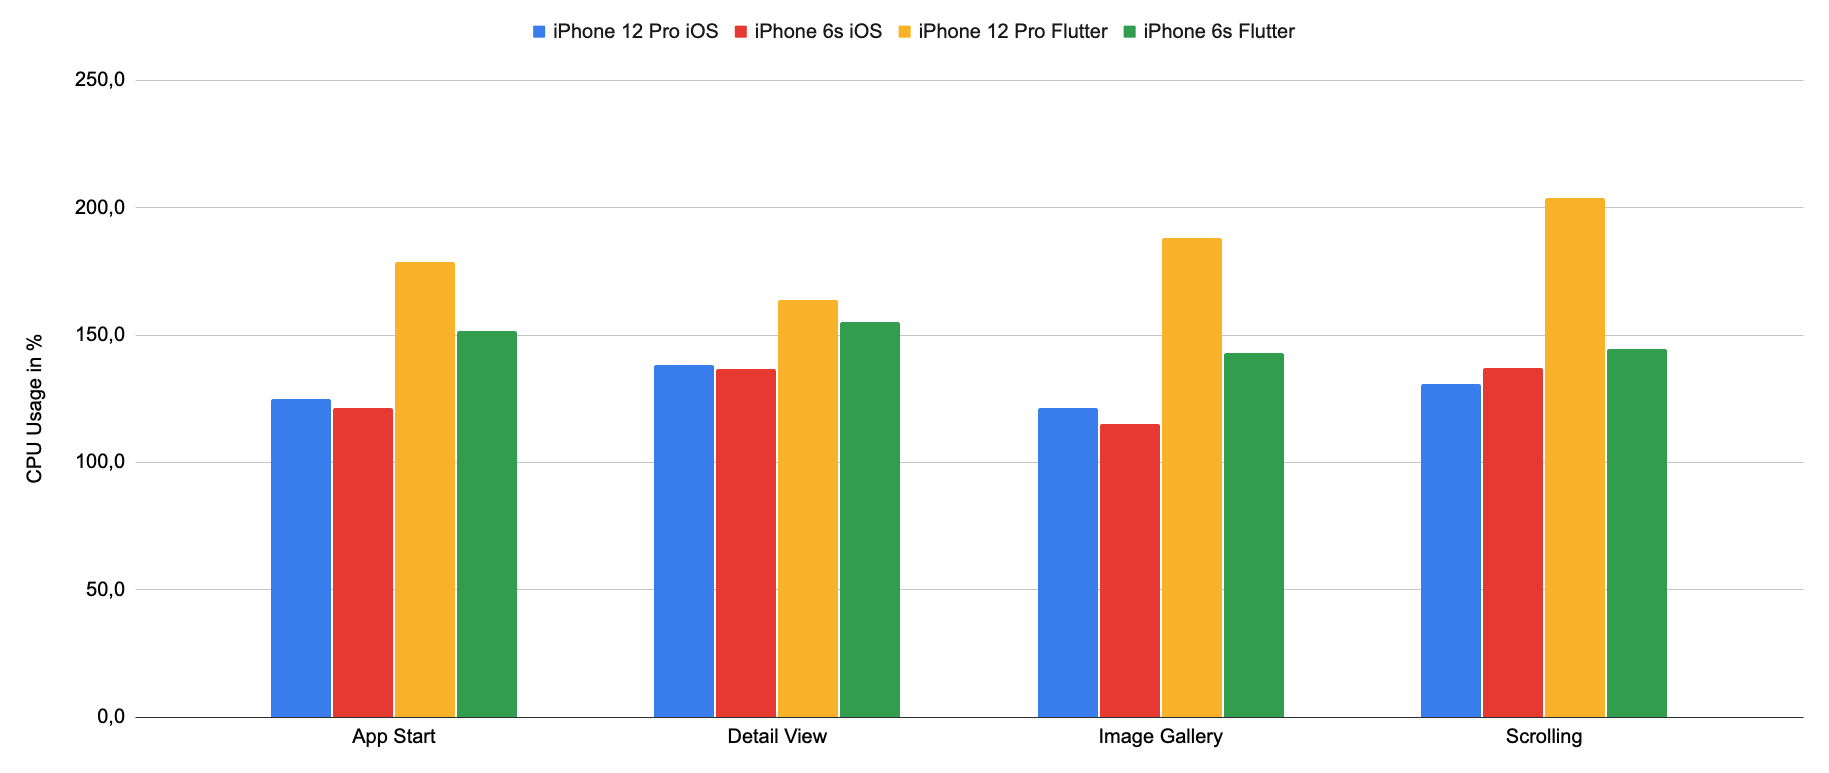
\includegraphics[width=\linewidth]{images/performance_results/summary_charts/avg_cpu_usage_summary.png}
    \caption{Averaged CPU Usage Summary}
    \label{fig:avg_cpu_usage_summary}
\end{figure}

\subsection{Memory Usage}
The memory usage grows quite steadily throughout the execution of each user action (as can be seen in Figures \ref{fig:avg_memory_usage_app_start}, \ref{fig:avg_memory_usage_detail_view}, \ref{fig:avg_memory_usage_image_gallery} and \ref{fig:avg_memory_usage_scrolling}) as opposed to the CPU usage (Section \ref{section::cpu_usage}).
When starting the application, a required amount of information is loaded into memory and 
as the use case is performed more information (i.e. more variables) are added into the memory units.\\
Flutter is less efficient in terms of its memory usage. Each use case consumes between 53.4 MiB\footnote{Mebibytes (MiB) are the base 2 equivalent (1,048,576) of Megabytes (MB) (1,000,000)} and 67.3 MiB of memory while the iOS baseline app only uses between 32.3 and 41.1 MiB of memory.
Thereby, the clone app uses double the amount of memory on average (124.7\% additional usage).
This may be explained by the fact, that the Flutter app contains its own rendering engine requiring additional space whereas the native rendering engine is built into the operating system itself.\\
However, the additional memory utilization the Flutter app requires (32.9 MiB) equates to 0.6\% and 1.7\% of the total RAM capacity for the 12 Pro Max and 6s\footnote{The iPhone 12 Pro Max has 6GB RAM (\cite{GSMArena12ProMax2020}) capacity while the iPhone 6s has 2GB RAM (\cite{GSMArena2015}) capacity} respectively.\\
Interestingly, the memory growth throughout each use case is smaller than on iOS (as can be seen in Figures \ref{fig:avg_memory_usage_app_start}, \ref{fig:avg_memory_usage_detail_view}, \ref{fig:avg_memory_usage_image_gallery} and \ref{fig:avg_memory_usage_scrolling}) indicating that Flutter efficiently scales memory during app runtime.
In addition, the additional 23.7 MiB the Flutter app consumes on average is negliglible as it is 0.4\% of the iPhone 12 Pro Max (6 GB) and 1.2\% of the 
iPhone 6s (2 GB) RAM capacity.

\begin{figure}[!h]
    \centering
    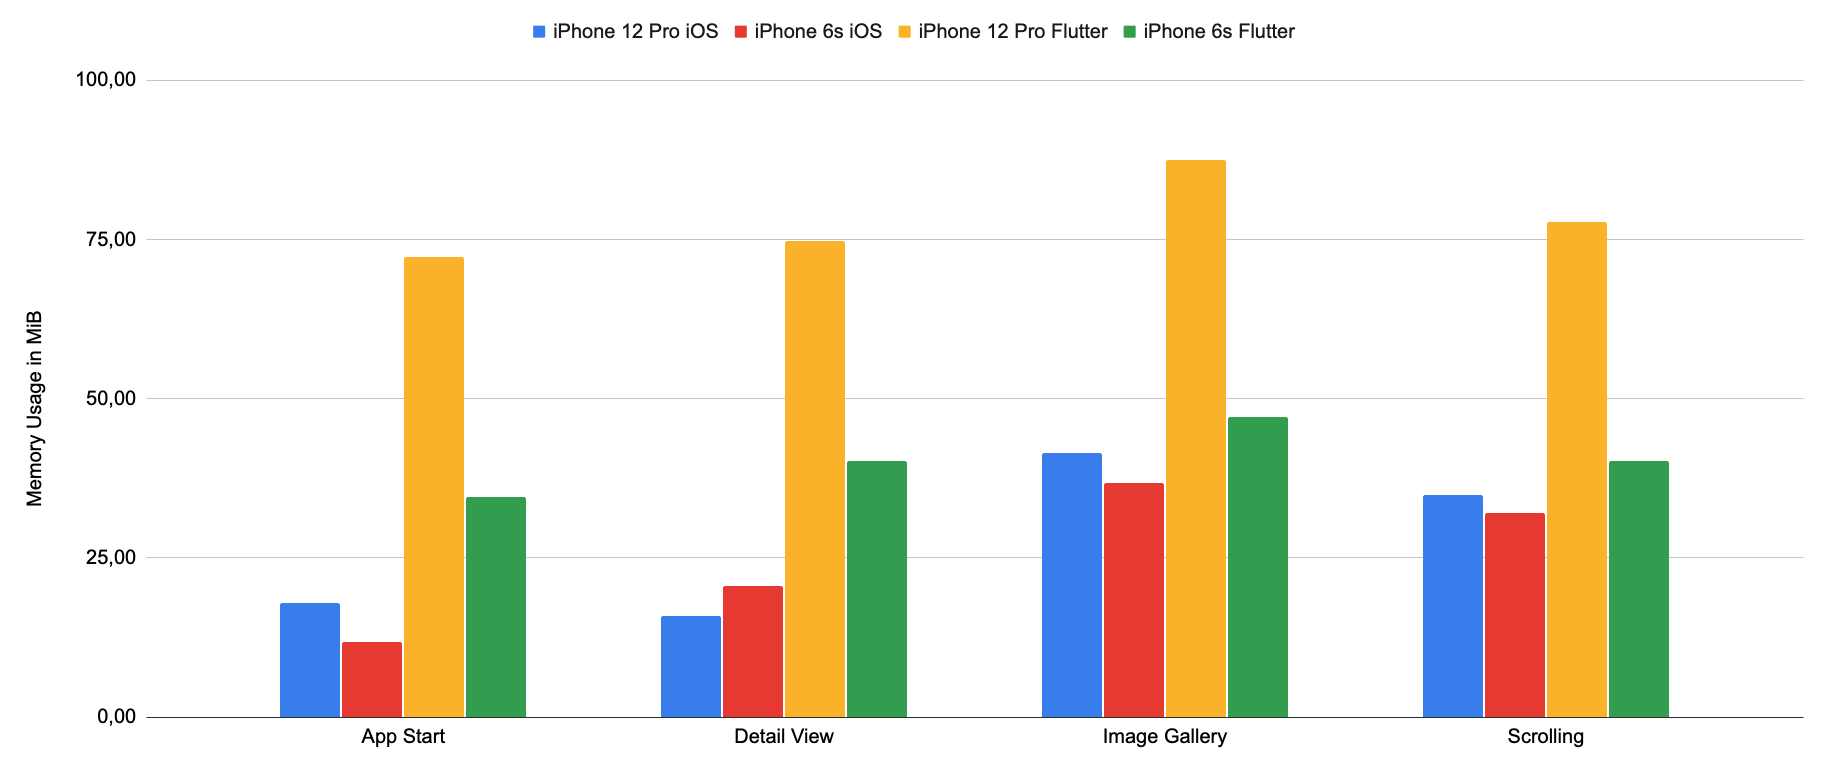
\includegraphics[width=\linewidth]{images/performance_results/summary_charts/avg_memory_usage_summary.png}
    \caption{Averaged Memory Usage Summary}
    \label{fig:avg_memory_usage_summary}
\end{figure}

\subsection{GPU Usage}
On average the Flutter app consumes 38\% more GPU than the Flutter application. The GPU usage lies between 18.7\% 21.9\% for Flutter and between 24.2\% and 37.4\% on iOS (averaged for each use case).
The Skia engine of the Flutter app (see Section \ref{section::flutter_architecture}) may use the CPU for certain calculations like tree diffing (being a typical CPU task, Section \ref{subsection::rendering_ui_state}) while iOS is optimized to perform graphics related calculations on the GPU.
This requirement inbalance may then also explain the additional CPU usage of the Flutter clone.\\
Furthermore, throughout each use case the iOS app is subject to larger gradient variation than the Flutter application (see Figures \ref{fig:avg_gpu_usage_app_start}, \ref{fig:avg_gpu_usage_detail_view}, \ref{fig:avg_gpu_usage_image_gallery} and \ref{fig:avg_gpu_usage_scrolling}).
This may be related to the fact that iOS demands more GPU usage at points in time where intensive graphical computations are required.

\begin{figure}[!h]
    \centering
    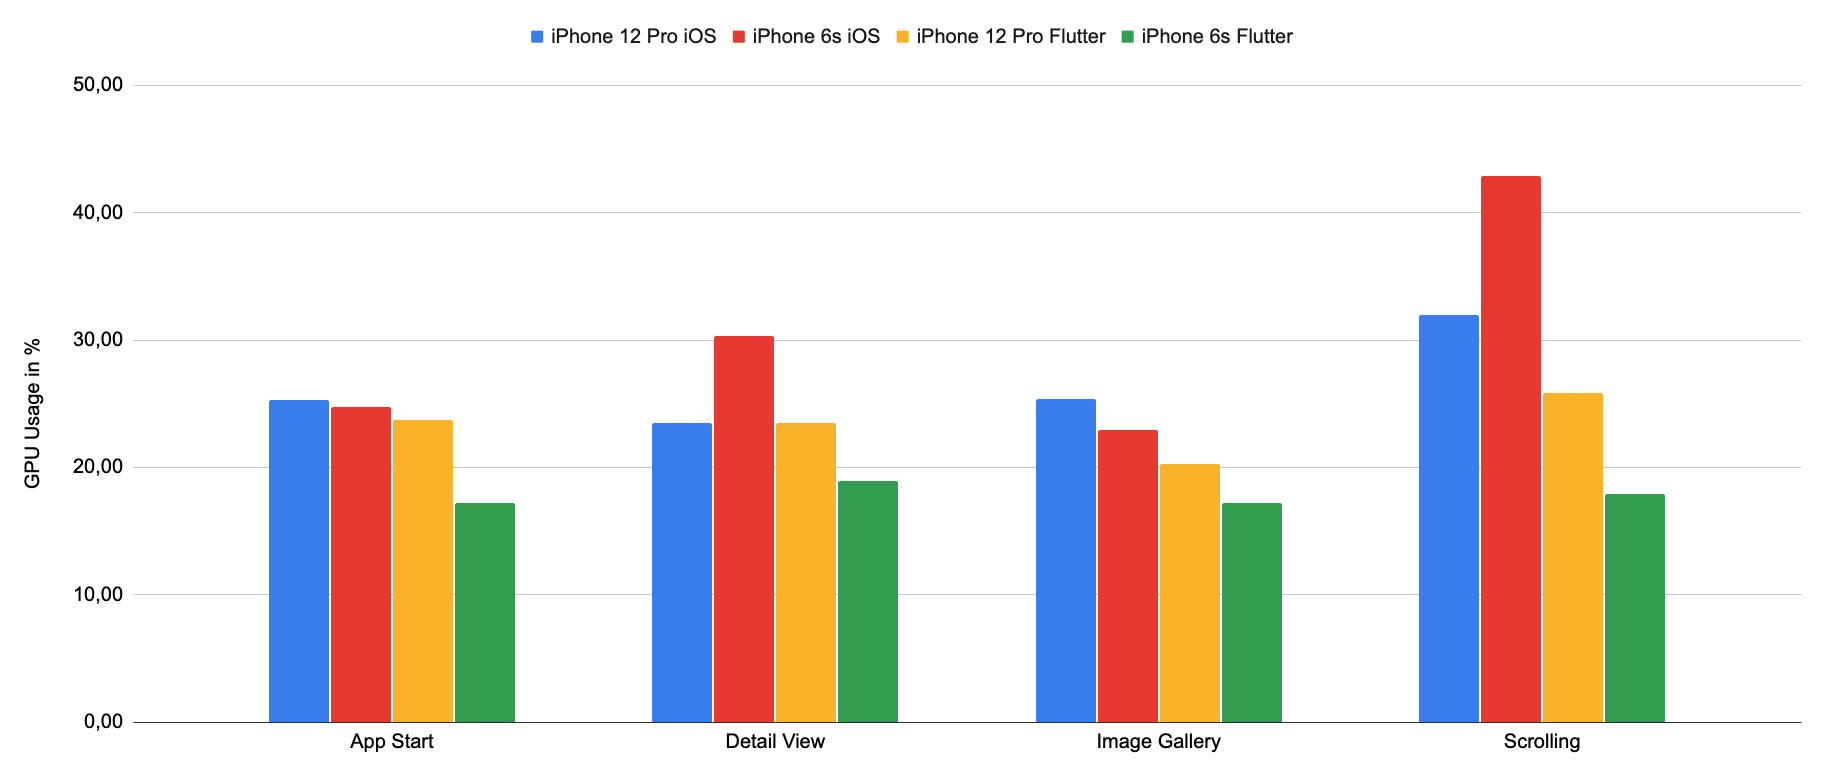
\includegraphics[width=\linewidth]{images/performance_results/summary_charts/avg_gpu_usage_summary.png}
    \caption{Averaged GPU Usage Summary}
    \label{fig:avg_gpu_usage_summary}
\end{figure}

\subsection{Hyptothesis Evaluation} \label{subsection::hypothesis_evaluation}
Overall, the Flutter application can be said to have a similar performance as iOS. The CPU usage is slightly worse while the GPU usage is slightly better for the Flutter app.
In relation, the memory usage is significantly higher in the Flutter clone. However, the relative memory usage for modern phones is sufficiently low and memory growth seems to be slower than
on iOS.

\section{Usability Comparison} \label{section::usability_comparison}
This section presents and contextualizes the results from the expert interview coding process (see Section \ref{section::interview_evaluation}).\\
In most cases the expert interview participants did not prefer either of the two user experiences as can be seen in Table \ref{tab:interview_use_case_preferences}.
Particularly, cases where no differences could be perceived include:
\begin{itemize}
    \item opening the application
    \item switch control interaction
    \item vertical scrolling on the overview page
    \item horizontal scrolling in the image gallery
\end{itemize}
Out of the above, cases 3 and 4 are presumably the most resource intensive UI operations out of all user actions as the collection items are dynamically fetched from a networked data source and are continuously rerendered based on the current users' scroll position.
Interestingly, the Flutter clone can provide the same perceived user experience as the iOS original.

When differences were noticed, the participants had to go through a particular use case multiple times in order to detect divergences between the two apps.
These could be categorized with the interview coding process (see Table \ref{tab:interview_coding_results}): \textit{Cross-Cutting differences}, \textit{Detail transition}, \textit{Modal transition}, \textit{Textfield keyboard animation}, \textit{Other specific differences}.\\
The following sections explain the above categories in detail.

\begin{table}[!htp]\centering
    \caption{Interview Use Case Cumulated Preference Choices}\label{tab:interview_use_case_preferences}
    \resizebox{\textwidth}{!}{%
        \begin{tabular}{lrrrrr}\toprule
        \textbf{Use Case} &\textbf{Preferred iOS App} &\textbf{Preffered Flutter App} &\textbf{Indifferent} &\textbf{Total} \\\midrule
        \textbf{App Start \& Scroll Behavior} &1 &0 &4 &5 \\
        \textbf{Detail Transition, Modal Transition, Textfield interaction} &4 &1 &0 &5 \\
        \textbf{Horizontal Scrolling} &1 &0 &4 &5 \\
        \textbf{Switch Control \& Web View} &0 &0 &5 &5 \\
        \bottomrule
        &6 &1 &13 & \\
        \midrule
    \end{tabular}}
\end{table}

\begin{table}[!htp]\centering
    \caption{Interview Coding Results}\label{tab:interview_coding_results}
    \scriptsize
    \begin{tabular}{lrr}\toprule
    \textbf{General differences} &Flutter App doesn't support dynamic type \\
    & \\
    \textbf{Detail Transition differences} &Flutter App has more interesting detail transition (mentioned twice) \\
    &iOS App uses typical navigation stack master-detail transition \\
    & \\
    \textbf{Modal Transition} &iOS App has more natural bottom sheet animation (mentioned thrice): \\
    &- Bottom Sheet is not draggable \\
    &- Animation curve of Flutter app is too linear \\
    \textbf{} & \\
    \textbf{Textfield interaction} &iOS keyboard animation feels more natural (mentioned twice \\
    &gap during keyboard animation \\
    & \\
    \textbf{Other specific differences} &Countdown Timer Spacing is slightly larger in Flutter \\
    &Status Bar Shadow is not implemented such that lighter images may be seen better \\
    &Webview close button title is different ("Schließen" vs "Fertig") \\
    &Alert dialog font letter spacing is larger in Flutter clone app \\
    & \\
    \bottomrule
    \end{tabular}
\end{table}

\subsection{Cross-Cutting Differences}
One participant noticed that the Flutter app did not have dynamic type support. 
Dynamic type is Apple's accessibility feature for users who need larger text for better readability based on their preferred system text size setting (\cite{Apple2021b}).
According to Google, Flutter scales \textit{Text} widgets automatically based on the respective OS setting (\cite{Google2021a}).
Upon further inspection, the Flutter app did scale its text, however the scaling factor seemed smaller than on iOS.

\subsection{Detail Transition}
The transition between the overview screen (Figure \ref{fig:kickdown_overview_screen}) and the detail screen (Figure \ref{fig:kickdown_detail_screen}) was implemented slightly differently in the Flutter application.
The exact navigation stack push/pop transitions of iOS are not yet integrated into the Cupertino package of Flutter. Therefore a custom transition was written for this screen transition.
One participant in the usability study noted that he could immediately detect the original app by this transition while two other participants actually preferred the transition in the Flutter clone.
Flutter is currently not able to fully mimic the native iOS navigation animation concept. However, transitions that multiple interview participants described as pleasant can be created with Flutter's integrated animation library.

\subsection{Modal Transition}
The default iOS modal presentation style implemented in the bid UI (see Figure \ref{fig:kickdown_bid_preparation_screen}) could not be fully replicated with Flutter as can be seen in Figure \ref{fig:bid_ui_iOS} and \ref{fig:bid_ui_flutter}.
Three out of the five participants noted this difference. 
They observed that the modally presented screen did not seem as natural as it was not draggable and its presentation animation curve appeared to be linear.\\
Flutter's animation system is rich enough to theoretically fully replicate the iOS modal screen transition. However, it would require a substantial amount of code as there are multiple animations 
running synchronously which may also reverse based on gestures. Furthermore, this process would involve a lot of trial and error since the original transition is closed source.
Ideally, the Flutter framework itself will replicate this screen transition and it can simply be set via an argument in the navigation function.

\begin{figure}[htbp]
    \begin{tabular}{p{0.33\textwidth}p{0.33\textwidth}p{0.33\textwidth}}
        \begin{minipage}{.33\textwidth}
            \centering
            \fbox{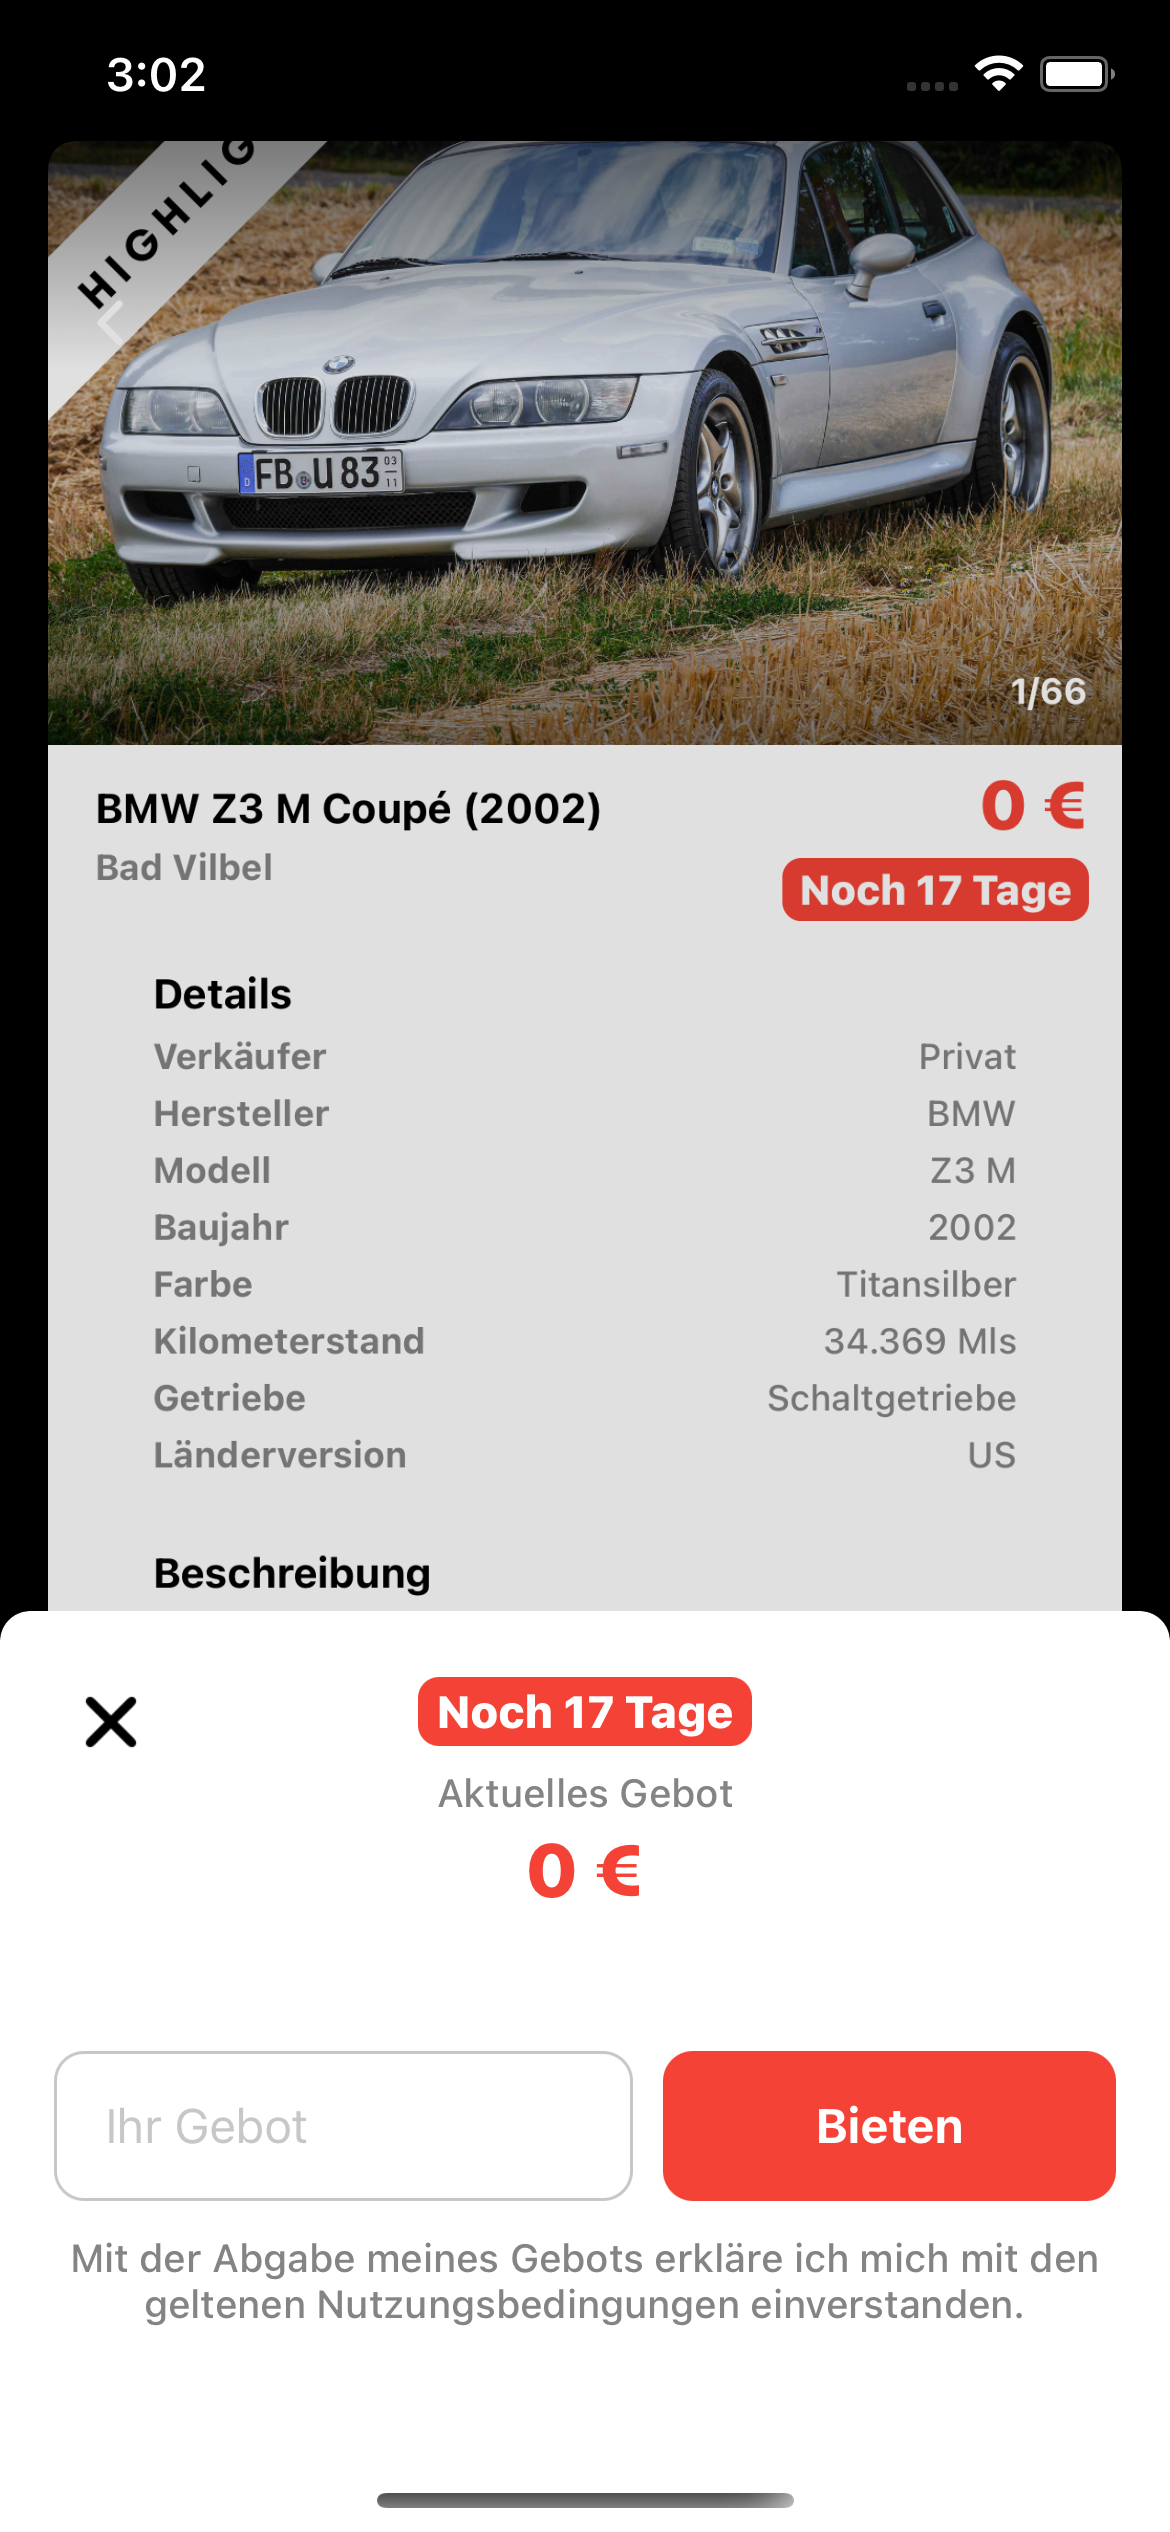
\includegraphics[width=\linewidth, height=300pt]{images/app_differences/bid_ui_iOS.PNG}}
            \caption{Bid UI iOS Original}
            \label{fig:bid_ui_iOS}
        \end{minipage}
        &
        \begin{minipage}{.33\textwidth}
            \centering
            \fbox{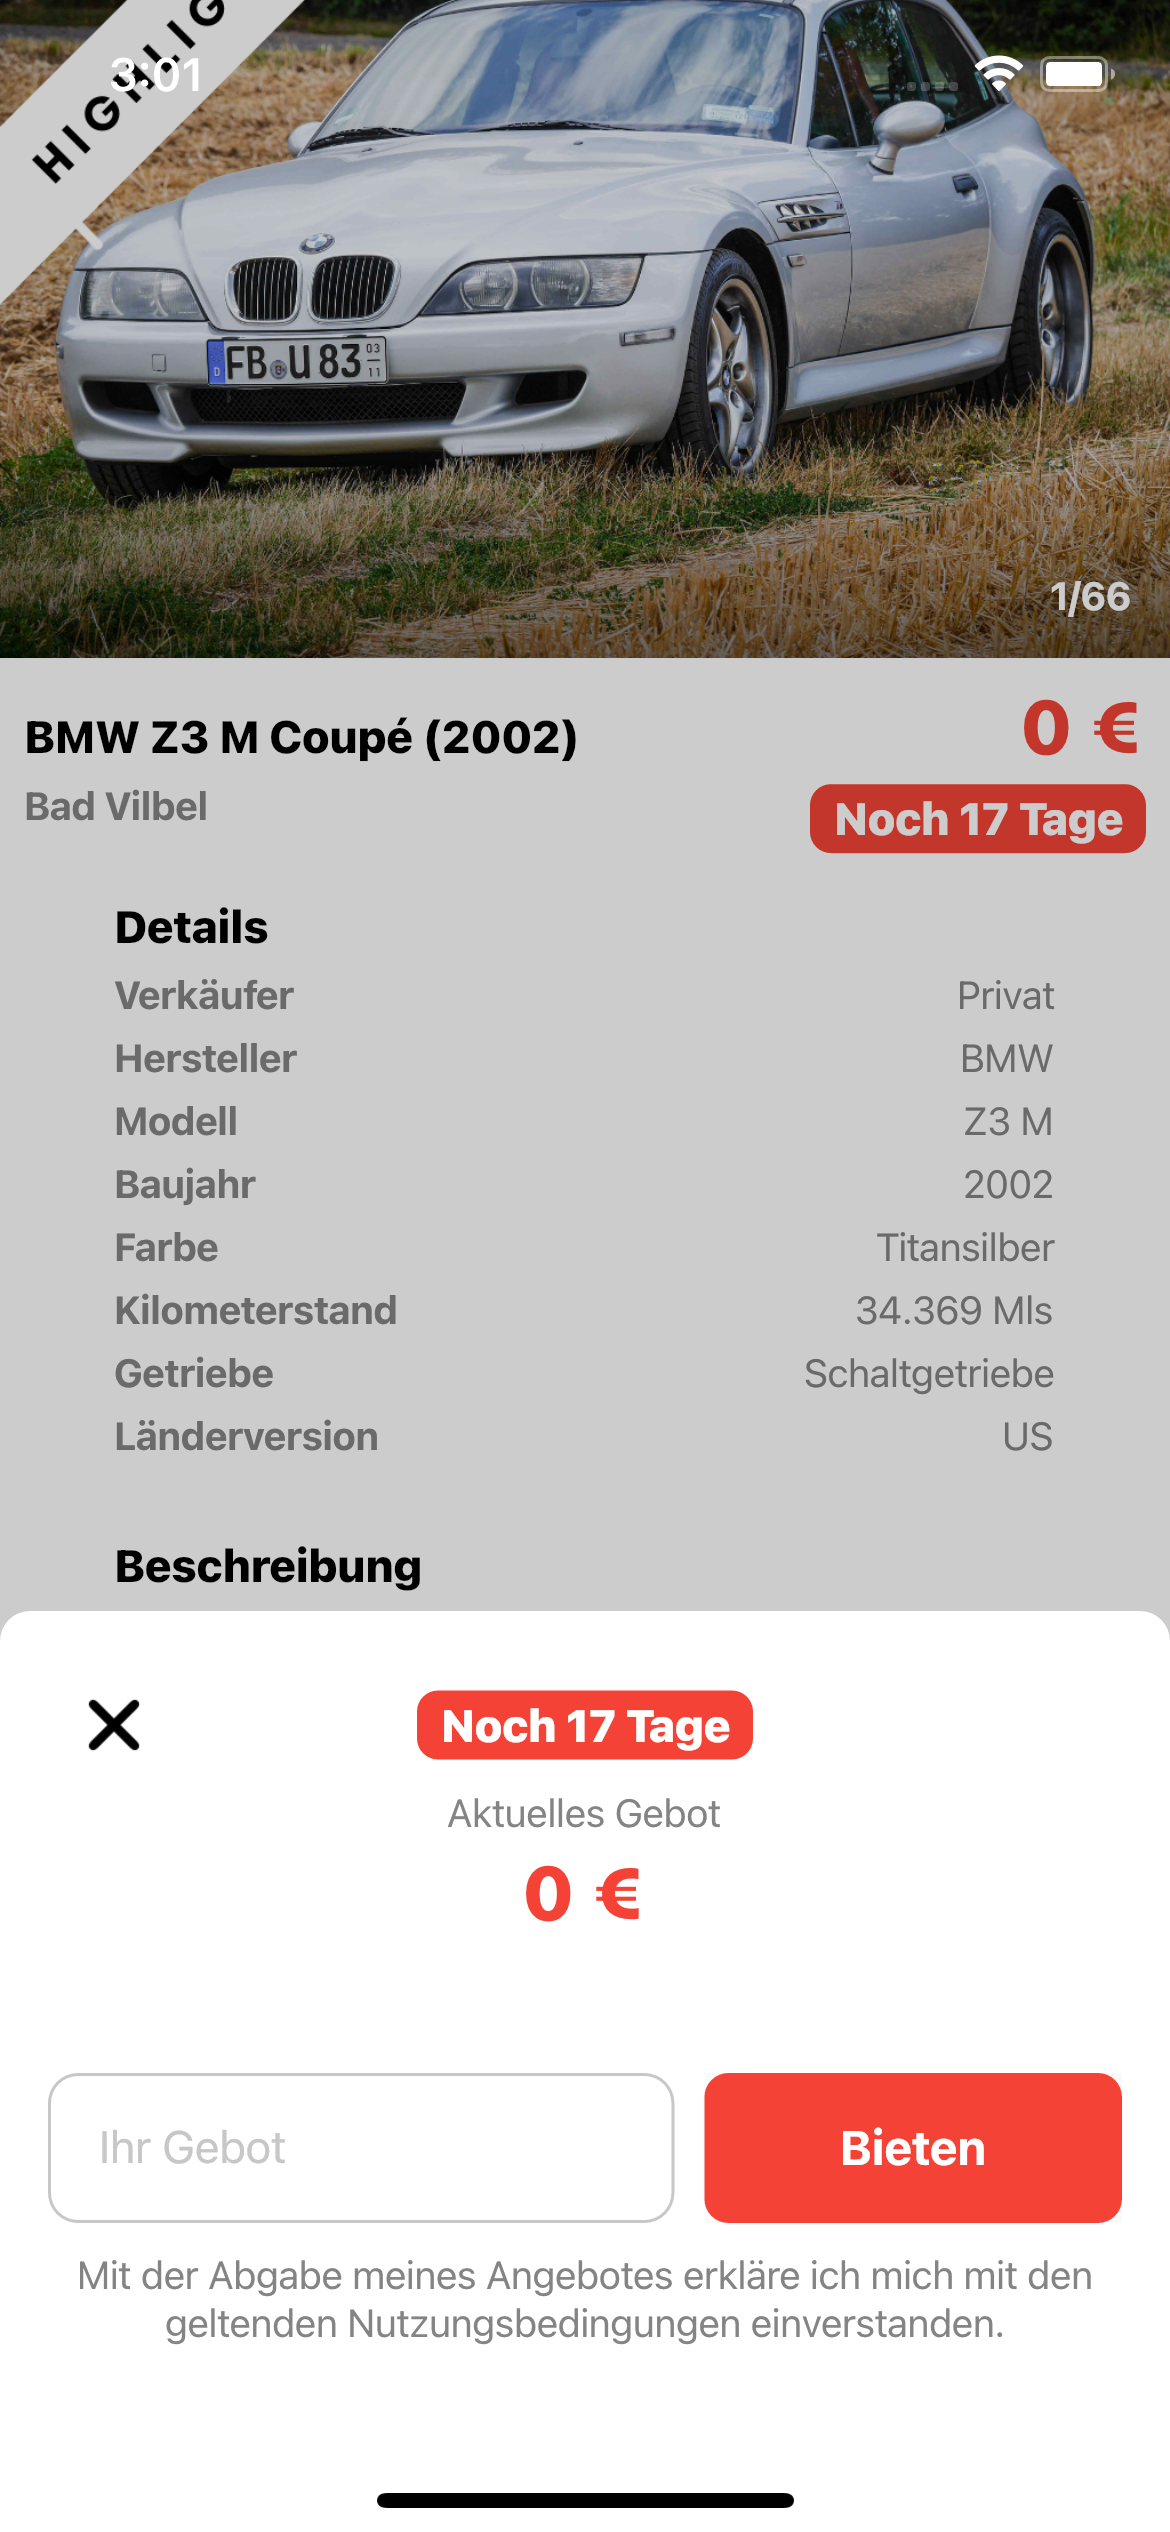
\includegraphics[width=\linewidth, height=300pt]{images/app_differences/bid_ui_Flutter.PNG}}
            \caption{Bid UI Flutter Clone}
            \label{fig:bid_ui_flutter}
        \end{minipage}
    \end{tabular}
\end{figure}


\subsection{Textfield Keyboard Animation}
When interacting with the textfield in the bid UI (see Figure \ref{fig:kickdown_bid_preparation_screen}), the keyboard automatically animates from the bottom for the user. The animation of the original iOS app felt more natural to three participants in the usability study. 
Further inspection of the Flutter app showed that the keyboard animation is slightly slower than the corresponding animation of the bottom sheet. The user expects that the keyboard pushes up the bottom sheet and they move synchronously, yet in the
Flutter app a small gap appears between the two elements for the animation duration due to unmatched speed of the two UI elements.
This difference wasn't noticed during the development of the clone application. The animation curve of the sheet may be changed while the keyboard transition is handled by the framework and not configurable. However, simply slowing
down the sheet transition should produce a comparable effect as in the original application.

\subsection{Other Specific Differences}
During the conduction of the interviews, individual participants noticed small but interesting differences between the two applications. These fall under the "Other Specific Differences" category resulting from the interview coding process and will be presented in this section.\\
One participant noted that the font letter spacing of the alert dialog of the Flutter application is slightly larger as can be seen in Figure \ref{fig:alert_dialog_iOS} and \ref{fig:alert_dialog_flutter}. 
The alert dialog of the Flutter Cupertino package doesn't implement the font correctly and an open Github issue exists since Feb 17, 2020 (\cite{FlutterCommunity2020}).\\
The other differences (see Table \ref{tab:interview_coding_results}) in this category were pointed out by a single participant and the implementation effort of correcting these differences in the Flutter clone are negligible.

\subsection{Usability Hypothesis Evaluation} \label{subsection::usability_hypothesis_evaluation}
Overall, Flutter can fully reconstruct native iOS user interfaces for typical mobile application facets. Furthermore, scrolling and animation fluidity is comparable with Flutter.\\
However, navigation animations for screen transitions
do not look and feel native for iOS users when building with Flutter. Additionally, the iOS system alert dialog styling is slightly different.

\begin{figure}[htbp]
    \begin{tabular}{p{0.33\textwidth}p{0.33\textwidth}p{0.33\textwidth}}
        \begin{minipage}{.33\textwidth}
            \centering
            \fbox{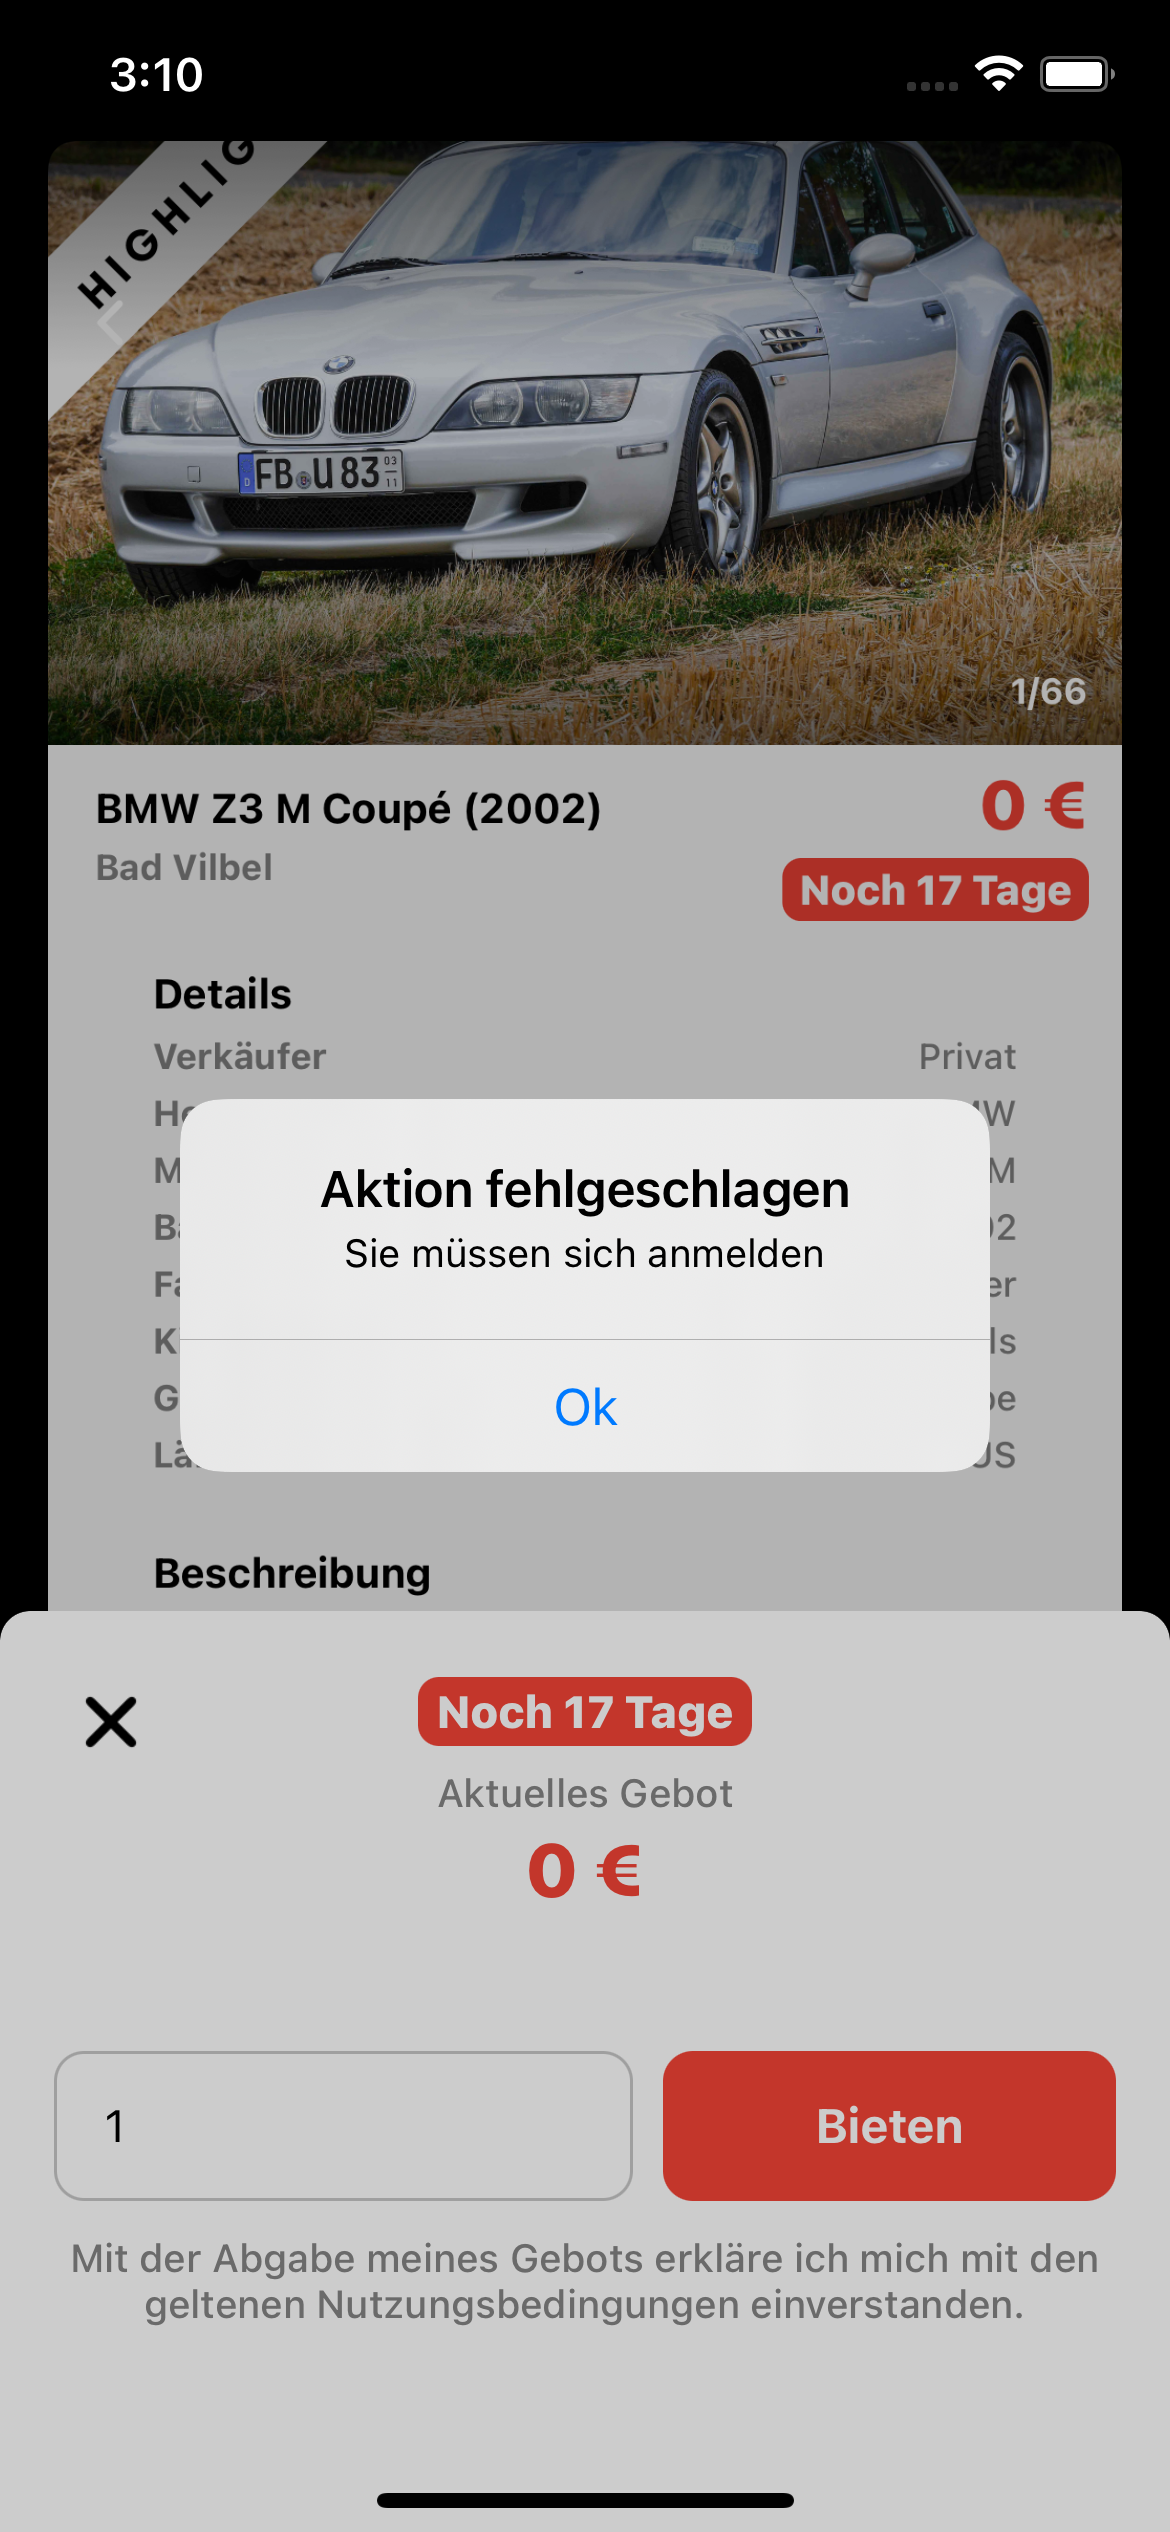
\includegraphics[width=\linewidth, height=300pt]{images/app_differences/alert_dialog_iOS.png}}
            \caption{Alert Dialog iOS Original}
            \label{fig:alert_dialog_iOS}
        \end{minipage}
        &
        \begin{minipage}{.33\textwidth}
            \centering
            \fbox{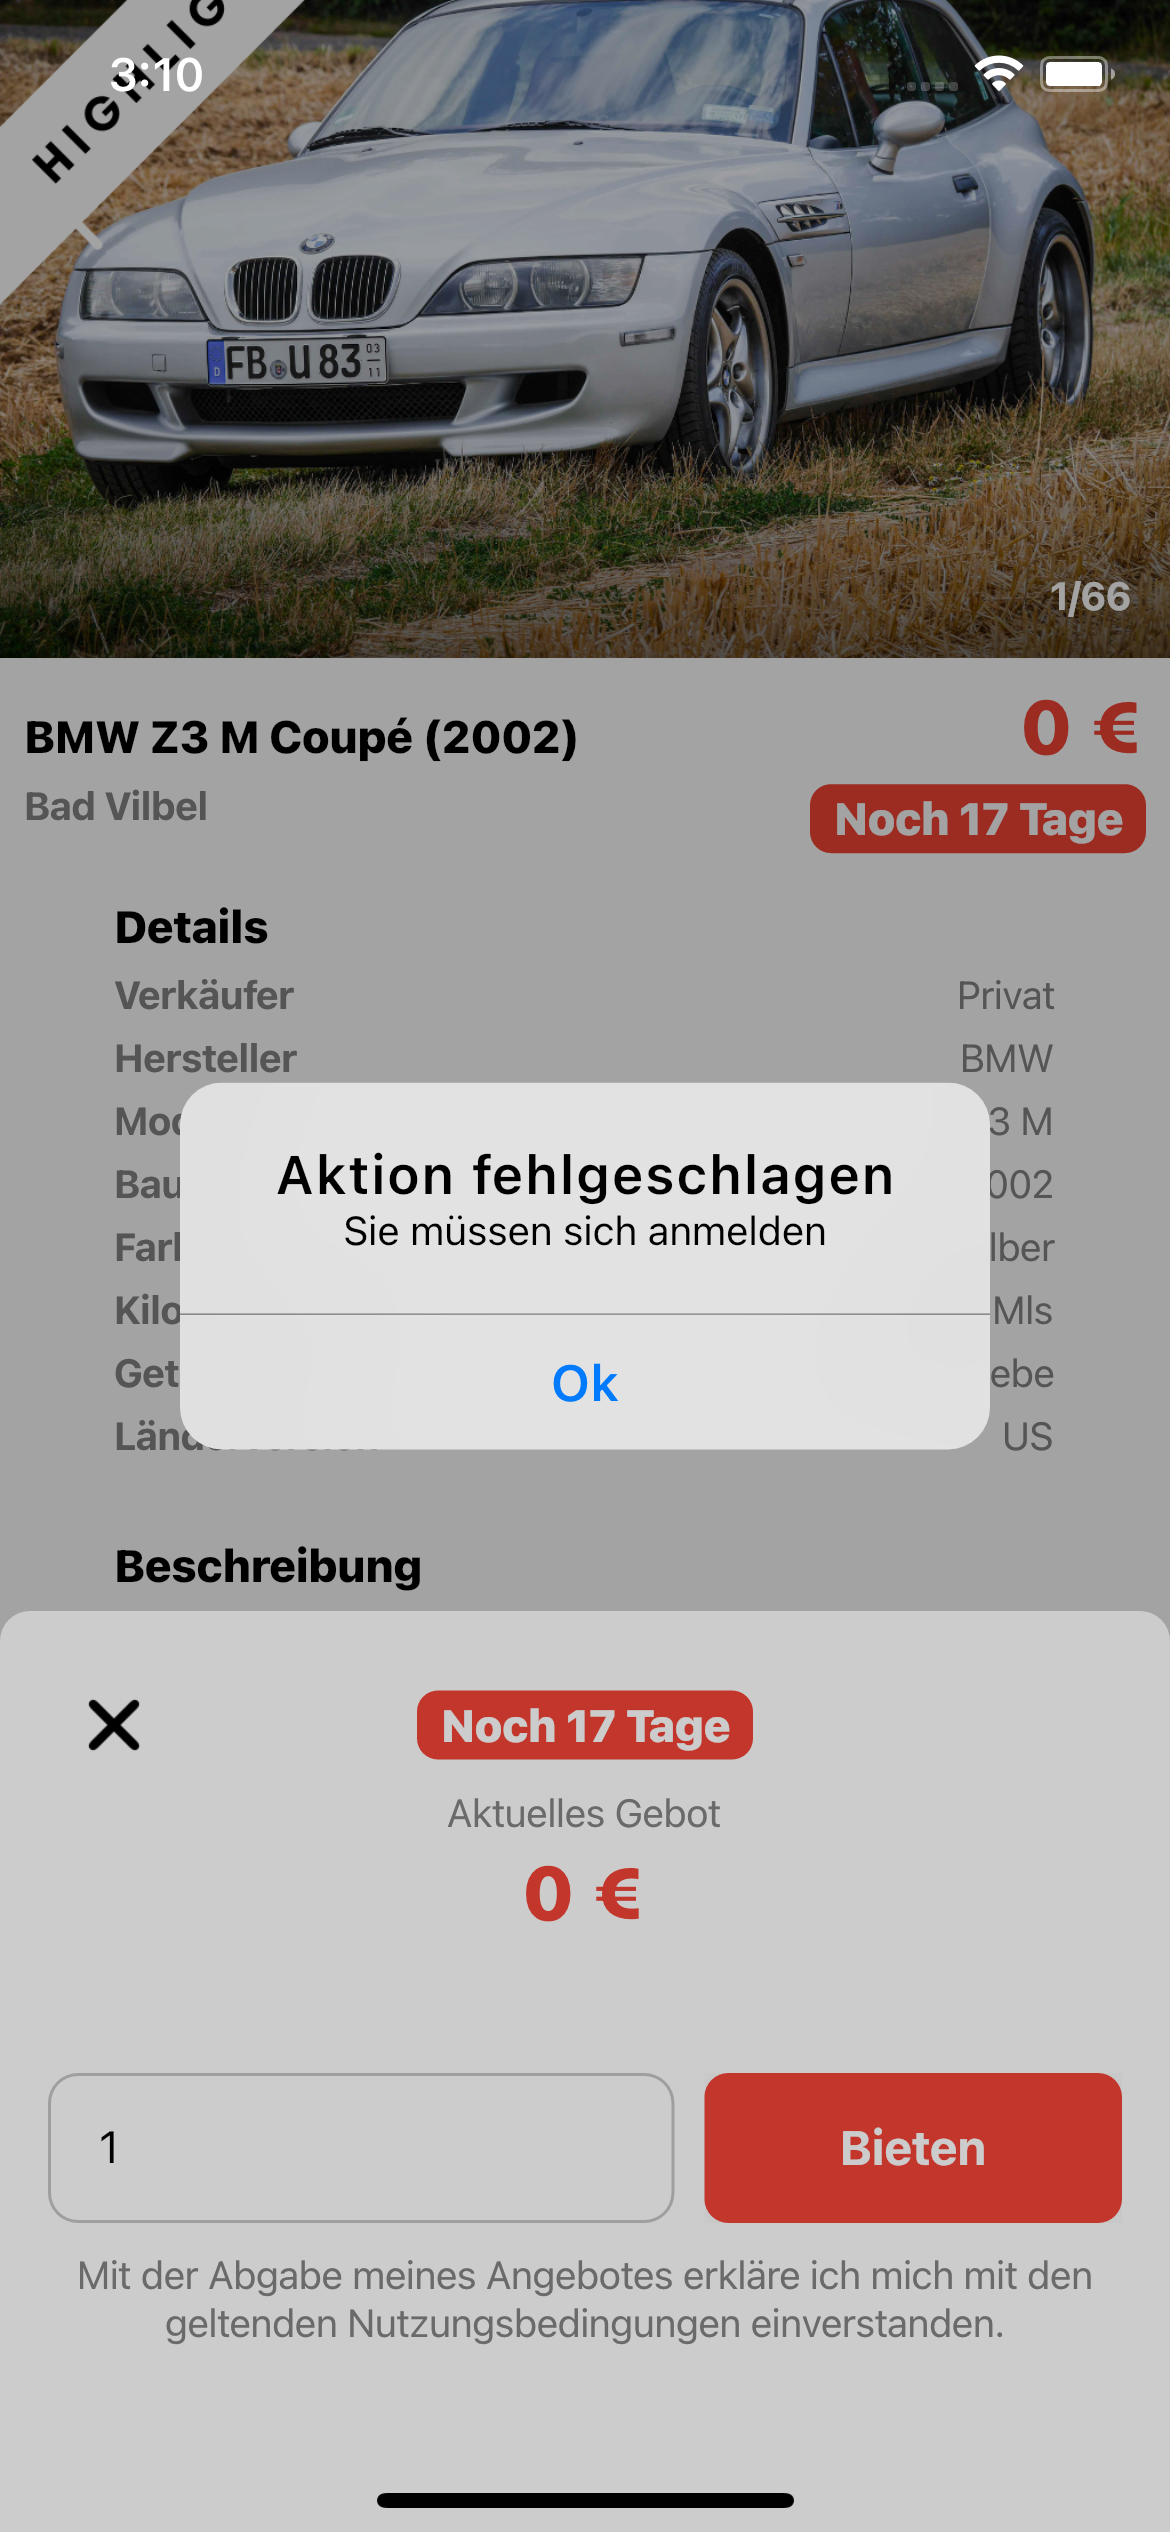
\includegraphics[width=\linewidth, height=300pt]{images/app_differences/alert_dialog_Flutter.png}}
            \caption{Alert Dialog Flutter Clone}
            \label{fig:alert_dialog_flutter}
        \end{minipage}
    \end{tabular}
\end{figure}